\documentclass{report}

\usepackage{graphicx}

\usepackage{amsfonts, amsmath, amssymb, amsthm}
\usepackage{bigfoot}
\usepackage{comment}
\usepackage[shortlabels]{enumitem}
\usepackage{etoolbox}
\usepackage{environ}
\usepackage{fontawesome5}
\usepackage{mathabx, mathrsfs}
\usepackage{soul}
\usepackage{stmaryrd}
% Must load `xcolor` before `tcolorbox` and `tikz`.
\usepackage[dvipsnames]{xcolor}
\usepackage{tcolorbox}
\usepackage{tikz}
% `hyperref` comes after `xr-hyper`.
\usepackage{xr-hyper}
\usepackage{hyperref}

% Open "private" namespace.
\makeatletter

% ========================================
% General
% ========================================

\newcommand{\header}[2]{\title{#1}\author{#2}\date{}\maketitle}

% ========================================
% Dividers
% ========================================

\newcommand\@linespace{\vspace{10pt}}
\newcommand\linedivider{\@linespace\hrule\@linespace}
\WithSuffix\newcommand\linedivider*{\@linespace\hrule}
\newcommand\suitdivider{$$\spadesuit\;\spadesuit\;\spadesuit$$}

% ========================================
% Linking
% ========================================

\hypersetup{colorlinks=true, linkcolor=blue, urlcolor=blue}
\newcommand{\textref}[1]{\text{\nameref{#1}}}
\newcommand{\hyperlabel}[1]{%
  \label{#1}%
  \hypertarget{#1}{}}

% Links to theorems/statements/etc. that can be found in Mathlib4's index.
\newcommand\@leanlink[3]{%
  \textcolor{BlueViolet}{\raisebox{-4.5pt}{%
    \tikz{\draw (0, 0) node[yscale=-1,xscale=1] {\faFont};}}{-\;}}%
  \href{https://leanprover-community.github.io/mathlib4_docs/#1.html\##2}%
  {\color{BlueViolet}{#3}}}

\newcommand\lean[2]{%
  \noindent\@leanlink{#1}{#2}{#2}}
\WithSuffix\newcommand\lean*[2]{%
  \vspace{6pt}\lean{#1}{#2}}

\newcommand\leanp[3]{%
  \noindent\@leanlink{#1}{#2}{#3}}
\WithSuffix\newcommand\leanp*[3]{%
  \vspace{6pt}\leanp{#1}{#2}{#3}}

% Links to theorems/statements/etc. found in custom index.
\newcommand\@codelink[4]{%
  \textcolor{MidnightBlue}{\raisebox{-4.5pt}{%
    \tikz{\draw (0, 0) node[xshift=8pt] {\faCodeBranch};}}{-\;}}%
  \href{#1/#2.html\##3}%
  {\color{MidnightBlue}{#4}}}

\newcommand\coderef[3]{%
  \@codelink{#1}{#2}{#3}{#3}}
\newcommand\codepref[4]{%
  \@codelink{#1}{#2}{#3}{#4}}

% Macro to build our `code` commands relative to a given directory. For
% instance, we expect to have invocation `\makecode{..}` if the TeX file exists
% one directory deep from the root of our project..
\newcommand\makecode[1]{%
  \newcommand\code[2]{%
    \noindent\coderef{#1}{##1}{##2}}
  \WithSuffix\newcommand\code*[2]{%
    \vspace{6pt}\noindent\coderef{#1}{##1}{##2}}

  \newcommand\codep[3]{%
    \noindent\codepref{#1}{##1}{##2}{##3}}
  \WithSuffix\newcommand\codep*[3]{%
    \vspace{6pt}\noindent\codepref{#1}{##1}{##2}{##3}}
}

% ========================================
% Admonitions
% ========================================

\NewEnviron{note}{%
  \begin{tcolorbox}[%
      sharp corners,
      fonttitle=\sffamily\bfseries,
      toptitle=2pt,
      bottomtitle=2pt,
      coltitle=black!80!white,
      colback=yellow!30,
      colframe=yellow!80!black,
      title=Note]
    \BODY
  \end{tcolorbox}}

% ========================================
% Statements
% ========================================

\newcommand\@statement[1]{%
  \linedivider*\paragraph{\normalfont\normalsize\textit{#1.}}}
\newenvironment{answer}{\@statement{Answer}}{\hfill$\square$}
\renewenvironment{proof}{\@statement{Proof}}{\hfill$\square$}

\newtheorem{corollaryinner}{Corollary}
\newenvironment{corollary}[1][]{%
  \ifstrempty{#1}
    {\corollaryinner}
    {\renewcommand\thecorollaryinner{#1}\corollaryinner}
}{\endcorollaryinner}

\newtheorem{lemmainner}{Lemma}
\newenvironment{lemma}[1][]{%
  \ifstrempty{#1}
    {\lemmainner}
    {\renewcommand\thelemmainner{#1}\lemmainner}
}{\endlemmainner}

\newtheorem{theoreminner}{Theorem}
\newenvironment{theorem}[1][]{%
  \ifstrempty{#1}
    {\theoreminner}
    {\renewcommand\thetheoreminner{#1}\theoreminner}
}{\endtheoreminner}

% ========================================
% Status
% ========================================

\DeclareRobustCommand{\defined}[1]{%
  \texorpdfstring{\color{darkgray}\faParagraph\ #1}{#1}}
\DeclareRobustCommand{\verified}[1]{%
  \texorpdfstring{\color{teal}\faCheckCircle\ #1}{#1}}
\DeclareRobustCommand{\unverified}[1]{%
  \texorpdfstring{\color{olive}\faCheckCircle[regular]\ #1}{#1}}
\DeclareRobustCommand{\pending}[1]{%
  \texorpdfstring{\color{Fuchsia}\faPencil*\ #1}{#1}}
\DeclareRobustCommand{\sorry}[1]{%
  \texorpdfstring{\color{Maroon}\faExclamationCircle\ #1}{#1}}

% ========================================
% Math
% ========================================

\newcommand{\abs}[1]{\left|#1\right|}
\newcommand{\ceil}[1]{\left\lceil#1\right\rceil}
\newcommand{\dom}[1]{\textop{dom}{#1}}
\newcommand{\fld}[1]{\textop{fld}{#1}}
\newcommand{\floor}[1]{\left\lfloor#1\right\rfloor}
\newcommand{\icc}[2]{\left[#1, #2\right]}
\newcommand{\ico}[2]{\left[#1, #2\right)}
\newcommand{\img}[2]{#1\!\left\llbracket#2\right\rrbracket}
\newcommand{\ioc}[2]{\left(#1, #2\right]}
\newcommand{\ioo}[2]{\left(#1, #2\right)}
\newcommand{\powerset}[1]{\mathscr{P}#1}
\newcommand{\ran}[1]{\textop{ran}{#1}}
\newcommand{\textop}[1]{\mathop{\text{#1}}}
\newcommand{\ubar}[1]{\text{\b{$#1$}}}

\let\oldemptyset\emptyset
\let\emptyset\varnothing

% Close off "private" namespace.
\makeatother


\graphicspath{{./Apostol/images/}}

\newcommand{\lean}[2]{\leanref{../#1.html\##2}{#2}}
\newcommand{\leanPretty}[3]{\leanref{../#1.html\##2}{#3}}

\begin{document}

\header
  {One-Variable Calculus, with an Introduction to Linear Algebra}
  {Tom M. Apostol}

\tableofcontents

\chapter{A Set of Axioms for the Real-Number System}%
\label{chap:set-axioms-real-number-system}

\section{\verified{Lemma 1}}%
\label{sec:lemma-1}

Nonempty set $S$ has supremum $L$ if and only if set $-S$ has infimum $-L$.

\begin{proof}

  \lean{Bookshelf/Apostol/Chapter\_I\_03}
    {Apostol.Chapter\_I\_03.is\_lub\_neg\_set\_iff\_is\_glb\_set\_neg}

  \divider

  Suppose $L = \sup{S}$ and fix $x \in S$.
  By definition of the supremum, $x \leq L$ and $L$ is the smallest value
    satisfying this inequality.
  Negating both sides of the inequality yields $-x \geq -L$.
  Furthermore, $-L$ must be the largest value satisfying this inequality.
  Therefore $-L = \inf{-S}$.

\end{proof}

\section{\verified{Theorem I.27}}%
\label{sec:theorem-i.27}

Every nonempty set $S$ that is bounded below has a greatest lower bound; that
  is, there is a real number $L$ such that $L = \inf{S}$.

\begin{proof}

  \lean{Bookshelf/Apostol/Chapter\_I\_03}
    {Apostol.Chapter\_I\_03.exists\_isGLB}

  \divider

  Let $S$ be a nonempty set bounded below by $x$.
  Then $-S$ is nonempty and bounded above by $x$.
  By the completeness axiom, there exists a supremum $L$ of $-S$.
  By \nameref{sec:lemma-1}, $L$ is a supremum of $-S$ if and only if $-L$ is an
    infimum of $S$.

\end{proof}

\section{\verified{Theorem I.29}}%
\label{sec:theorem-i.29}

For every real $x$ there exists a positive integer $n$ such that $n > x$.

\begin{proof}

  \lean{Bookshelf/Apostol/Chapter\_I\_03}
    {Apostol.Chapter\_I\_03.exists\_pnat\_geq\_self}

  \divider

  Let $n = \abs{\ceil{x}} + 1$.
  It is trivial to see $n$ is a positive integer satisfying $n \geq 1$.
  Thus all that remains to be shown is that $n > x$.
  If $x$ is nonpositive, $n > x$ immediately follows from $n \geq 1$.
  If $x$ is positive,
    $$x = \abs{x} \leq \abs{\ceil{x}} < \abs{\ceil{x}} + 1 = n.$$

\end{proof}

\section{\verified{Theorem I.30}}%
\label{sec:theorem-i.30}

If $x > 0$ and if $y$ is an arbitrary real number, there exists a positive
  integer $n$ such that $nx > y$.

\note{This is known as the "Archimedean Property of the Reals."}

\begin{proof}

  \lean{Bookshelf/Apostol/Chapter\_I\_03}
    {Apostol.Chapter\_I\_03.exists\_pnat\_mul\_self\_geq\_of\_pos}

  \divider

  Let $x > 0$ and $y$ be an arbitrary real number.
  By \nameref{sec:theorem-i.29}, there exists a positive integer $n$ such that
    $n > y / x$.
  Multiplying both sides of the inequality yields $nx > y$ as expected.

\end{proof}

\section{\verified{Theorem I.31}}%
\label{sec:theorem-i.31}

If three real numbers $a$, $x$, and $y$ satisfy the inequalities
  $$a \leq x \leq a + \frac{y}{n}$$ for every integer $n \geq 1$, then $x = a$.

\begin{proof}

  \lean{Bookshelf/Apostol/Chapter\_I\_03}
    {Apostol.Chapter\_I\_03.forall\_pnat\_leq\_self\_leq\_frac\_imp\_eq}

  \divider

  By the trichotomy of the reals, there are three cases to consider:

  \paragraph{Case 1}%

    Suppose $x = a$.
    Then we are immediately finished.

  \paragraph{Case 2}%

    Suppose $x < a$.
    But by hypothesis, $a \leq x$.
    Thus $a < a$, a contradiction.

  \paragraph{Case 3}%

    Suppose $x > a$.
    Then there exists some $c > 0$ such that $a + c = x$.
    By \nameref{sec:theorem-i.30}, there exists an integer $n > 0$ such that
      $nc > y$.
    Rearranging terms, we see $y / n < c$.
    Therefore $a + y / n < a + c = x$.
    But by hypothesis, $x \leq a + y / n$.
    Thus $a + y / n < a + y / n$, a contradiction.

  \paragraph{Conclusion}%

    Since these cases are exhaustive and both case 2 and 3 lead to
      contradictions, $x = a$ is the only possibility.

\end{proof}

\section{\verified{Lemma 2}}%
\label{sec:lemma-2}

If three real numbers $a$, $x$, and $y$ satisfy the inequalities
  $$a - y / n \leq x \leq a$$ for every integer $n \geq 1$, then $x = a$.

\begin{proof}

  \lean{Bookshelf/Apostol/Chapter\_I\_03}
    {Apostol.Chapter\_I\_03.forall\_pnat\_frac\_leq\_self\_leq\_imp\_eq}

  \divider

  By the trichotomy of the reals, there are three cases to consider:

  \paragraph{Case 1}%

    Suppose $x = a$.
    Then we are immediately finished.

  \paragraph{Case 2}%

    Suppose $x < a$.
    Then there exists some $c > 0$ such that $x = a - c$.
    By \nameref{sec:theorem-i.30}, there exists an integer $n > 0$ such that
      $nc > y$.
    Rearranging terms, we see that $y / n < c$.
    Therefore $a - y / n > a - c = x$.
    But by hypothesis, $x \geq a - y / n$.
    Thus $a - y / n < a - y / n$, a contradiction.

  \paragraph{Case 3}%

    Suppose $x > a$.
    But by hypothesis $x \leq a$.
    Thus $a < a$, a contradiction.

  \paragraph{Conclusion}%

    Since these cases are exhaustive and both case 2 and 3 lead to
      contradictions, $x = a$ is the only possibility.

\end{proof}

\section{Theorem I.32}%
\label{sec:theorem-i.32}

Let $h$ be a given positive number and let $S$ be a set of real numbers.

\subsection{\verified{Theorem I.32a}}%
\label{sub:theorem-i.32a}

If $S$ has a supremum, then for some $x$ in $S$ we have $x > \sup{S} - h$.

\begin{proof}

  \lean{Bookshelf/Apostol/Chapter\_I\_03}
    {Apostol.Chapter\_I\_03.sup\_imp\_exists\_gt\_sup\_sub\_delta}

  \divider

  By definition of a supremum, $\sup{S}$ is the least upper bound of $S$.
  For the sake of contradiction, suppose for all $x \in S$,
    $x \leq \sup{S} - h$.
  This immediately implies $\sup{S} - h$ is an upper bound of $S$.
  But $\sup{S} - h < \sup{S}$, contradicting $\sup{S}$ being the \textit{least}
    upper bound.
  Therefore our original hypothesis was wrong.
  That is, there exists some $x \in S$ such that $x > \sup{S} - h$.

\end{proof}

\subsection{\verified{Theorem I.32b}}%
\label{sub:theorem-i.32b}

If $S$ has an infimum, then for some $x$ in $S$ we have $x < \inf{S} + h$.

\begin{proof}

  \lean{Bookshelf/Apostol/Chapter\_I\_03}
    {Apostol.Chapter\_I\_03.inf\_imp\_exists\_lt\_inf\_add\_delta}

  \divider

  By definition of an infimum, $\inf{S}$ is the greatest lower bound of $S$.
  For the sake of contradiction, suppose for all $x \in S$,
    $x \geq \inf{S} + h$.
  This immediately implies $\inf{S} + h$ is a lower bound of $S$.
  But $\inf{S} + h > \inf{S}$, contradicting $\inf{S}$ being the
    \textit{greatest} lower bound.
  Therefore our original hypothesis was wrong.
  That is, there exists some $x \in S$ such that $x < \inf{S} + h$.

\end{proof}

\section{Theorem I.33}%
\label{sec:theorem-i.33}

Given nonempty subsets $A$ and $B$ of $\mathbb{R}$, let $C$ denote the set
  $$C = \{a + b : a \in A, b \in B\}.$$

\note{This is known as the "Additive Property."}

\subsection{\verified{Theorem I.33a}}%
\label{sub:theorem-i.33a}

If each of $A$ and $B$ has a supremum, then $C$ has a supremum, and
  $$\sup{C} = \sup{A} + \sup{B}.$$

\begin{proof}

  \lean{Bookshelf/Apostol/Chapter\_I\_03}
    {Apostol.Chapter\_I\_03.sup\_minkowski\_sum\_eq\_sup\_add\_sup}

  \divider

  We prove (i) $\sup{A} + \sup{B}$ is an upper bound of $C$ and (ii)
    $\sup{A} + \sup{B}$ is the \textit{least} upper bound of $C$.

  \paragraph{(i)}%
  \label{par:theorem-i.33a-i}

    Let $x \in C$.
    By definition of $C$, there exist elements $a' \in A$ and $b' \in B$ such
      that $x = a' + b'$.
    By definition of a supremum, $a' \leq \sup{A}$.
    Likewise, $b' \leq \sup{B}$.
    Therefore $a' + b' \leq \sup{A} + \sup{B}$.
    Since $x = a' + b'$ was arbitrarily chosen, it follows $\sup{A} + \sup{B}$
      is an upper bound of $C$.

  \paragraph{(ii)}%

    Since $A$ and $B$ have supremums, $C$ is nonempty.
    By \nameref{par:theorem-i.33a-i}, $C$ is bounded above.
    Therefore the completeness axiom tells us $C$ has a supremum.
    Let $n > 0$ be an integer.
    We now prove that
      \begin{equation}
        \label{par:theorem-i.33a-ii-eq1}
        \sup{C} \leq \sup{A} + \sup{B} \leq \sup{C} + 1 / n.
      \end{equation}

    \subparagraph{Left-Hand Side}%

      First consider the left-hand side of \eqref{par:theorem-i.33a-ii-eq1}.
      By \nameref{par:theorem-i.33a-i}, $\sup{A} + \sup{B}$ is an upper bound of
        $C$.
      Since $\sup{C}$ is the \textit{least} upper bound of $C$, it follows
        $\sup{C} \leq \sup{A} + \sup{B}$.

    \subparagraph{Right-Hand Side}%

      Next consider the right-hand side of \eqref{par:theorem-i.33a-ii-eq1}.
      By \nameref{sub:theorem-i.32a}, there exists some $a' \in A$ such that
        $\sup{A} < a' + 1 / (2n)$.
      Likewise, there exists some $b' \in B$ such that
        $\sup{B} < b' + 1 / (2n)$.
      Adding these two inequalities together shows
        \begin{align*}
          \sup{A} + \sup{B}
            & < a' + b' + 1 / n \\
            & \leq \sup{C} + 1 / n.
        \end{align*}

    \subparagraph{Conclusion}%

      Applying \nameref{sec:theorem-i.31} to \eqref{par:theorem-i.33a-ii-eq1}
        proves $\sup{C} = \sup{A} + \sup{B}$ as expected.

\end{proof}

\subsection{\verified{Theorem I.33b}}%
\label{sub:theorem-i.33b}

If each of $A$ and $B$ has an infimum, then $C$ has an infimum, and
  $$\inf{C} = \inf{A} + \inf{B}.$$

\begin{proof}

  \lean{Bookshelf/Apostol/Chapter\_I\_03}
    {Apostol.Chapter\_I\_03.inf\_minkowski\_sum\_eq\_inf\_add\_inf}

  \divider

  We prove (i) $\inf{A} + \inf{B}$ is a lower bound of $C$ and (ii)
    $\inf{A} + \inf{B}$ is the \textit{greatest} lower bound of $C$.

  \paragraph{(i)}%
  \label{par:theorem-i.33b-i}

    Let $x \in C$.
    By definition of $C$, there exist elements $a' \in A$ and $b' \in B$ such
      that $x = a' + b'$.
    By definition of an infimum, $a' \geq \inf{A}$.
    Likewise, $b' \geq \inf{B}$.
    Therefore $a' + b' \geq \inf{A} + \inf{B}$.
    Since $x = a' + b'$ was arbitrarily chosen, it follows $\inf{A} + \inf{B}$
      is a lower bound of $C$.

  \paragraph{(ii)}%

    Since $A$ and $B$ have infimums, $C$ is nonempty.
    By \nameref{par:theorem-i.33b-i}, $C$ is bounded below.
    Therefore \nameref{sec:theorem-i.27} tells us $C$ has an infimum.
    Let $n > 0$ be an integer.
    We now prove that
      \begin{equation}
        \label{par:theorem-i.33b-ii-eq1}
        \inf{C} - 1 / n \leq \inf{A} + \inf{B} \leq \inf{C}.
      \end{equation}

    \subparagraph{Right-Hand Side}%

      First consider the right-hand side of \eqref{par:theorem-i.33b-ii-eq1}.
      By \nameref{par:theorem-i.33b-i}, $\inf{A} + \inf{B}$ is a lower bound of
        $C$.
      Since $\inf{C}$ is the \textit{greatest} upper bound of $C$, it follows
        $\inf{C} \geq \inf{A} + \inf{B}$.

    \subparagraph{Left-Hand Side}%

      Next consider the left-hand side of \eqref{par:theorem-i.33b-ii-eq1}.
      By \nameref{sub:theorem-i.32b}, there exists some $a' \in A$ such that
        $\inf{A} > a' - 1 / (2n)$.
      Likewise, there exists some $b' \in B$ such that
        $\inf{B} > b' - 1 / (2n)$.
      Adding these two inequalities together shows
        \begin{align*}
          \inf{A} + \inf{B}
            & > a' + b' - 1 / n \\
            & \geq \inf{C} - 1 / n.
        \end{align*}

    \subparagraph{Conclusion}%

      Applying \nameref{sec:lemma-2} to \eqref{par:theorem-i.33b-ii-eq1}
        proves $\inf{C} = \inf{A} + \inf{B}$ as expected.

\end{proof}

\section{\verified{Theorem I.34}}%
\label{sec:theorem-i.34}

Given two nonempty subsets $S$ and $T$ of $\mathbb{R}$ such that $$s \leq t$$
  for every $s$ in $S$ and every $t$ in $T$. Then $S$ has a supremum, and $T$
  has an infimum, and they satisfy the inequality $$\sup{S} \leq \inf{T}.$$

\begin{proof}

  \lean{Bookshelf/Apostol/Chapter\_I\_03}
    {Apostol.Chapter\_I\_03.forall\_mem\_le\_forall\_mem\_imp\_sup\_le\_inf}

  \divider

  By hypothesis, $S$ and $T$ are nonempty sets.
  Let $s \in S$ and $t \in T$.
  Then $t$ is an upper bound of $S$ and $s$ is a lower bound of $T$.
  By the completeness axiom, $S$ has a supremum.
  By \nameref{sec:theorem-i.27}, $T$ has an infimum.
  All that remains is showing $\sup{S} \leq \inf{T}$.

  For the sake of contradiction, suppose $\sup{S} > \inf{T}$.
  Then there exists some $c > 0$ such that $\sup{S} = \inf{T} + c$.
  Therefore $\inf{T} < \sup{S} - c / 2$.
  By \nameref{sub:theorem-i.32a}, there exists some $x \in S$ such that
    $\sup{S} - c / 2 < x$.
  Thus $$\inf{T} < \sup{S} - c / 2 < x.$$
  But by hypothesis, $x \in S$ is a lower bound of $T$ meaning $x \leq \inf{T}$.
  Therefore $x < x$, a contradiction.
  Out original assumption is incorrect; that is, $\sup{S} \leq \inf{T}$.

\end{proof}

\chapter{The Concept of Area as a Set Function}%
\label{chap:concept-area-set-function}

We assume there exists a class $\mathscr{M}$ of measurable sets in the plane and
  a set function $a$, whose domain is $\mathscr{M}$, with the following
  properties:

\section{\defined{Nonnegative Property}}%
\label{sec:nonnegative-property}

For each set $S$ in $\mathscr{M}$, we have $a(S) \geq 0$.

\begin{axiom}

  \leanPretty{Common/Real/Geometry/Area}{Nonnegative-Property}
    {Nonnegative Property}

\end{axiom}

\section{\defined{Additive Property}}%
\label{sec:additive-property}

If $S$ and $T$ are in $\mathscr{M}$, then $S \cup T$ and $S \cap T$ are in
  $\mathscr{M}$, and we have $a(S \cup T) = a(S) + a(T) - a(S \cap T)$.

\begin{axiom}

  \leanPretty{Common/Real/Geometry/Area}{Additive-Property}
    {Additive Property}

\end{axiom}

\section{\defined{Difference Property}}%
\label{sec:difference-property}

If $S$ and $T$ are in $\mathscr{M}$ with $S \subseteq T$, then $T - S$ is in
  $\mathscr{M}$, and we have $a(T - S) = a(T) - a(S)$.

\begin{axiom}

  \leanPretty{Common/Real/Geometry/Area}{Difference-Property}
    {Difference Property}

\end{axiom}

\section{\defined{Invariance Under Congruence}}%
\label{sec:invariance-under-congruence}

If a set $S$ is in $\mathscr{M}$ and if $T$ is congruent to $S$, then $T$ is
  also in $\mathscr{M}$ and we have $a(S) = a(T)$.

\begin{axiom}

  \leanPretty{Common/Real/Geometry/Area}{Invariance-Under-Congruence}
    {Invariance Under Congruence}

\end{axiom}

\section{\defined{Choice of Scale}}%
\label{sec:choice-scale}

Every rectangle $R$ is in $\mathscr{M}$.
If the edges of $R$ have lengths $h$ and $k$, then $a(R) = hk$.

\begin{axiom}

  \leanPretty{Common/Real/Geometry/Area}{Choice-of-Scale}
    {Choice of Scale}

\end{axiom}

\section{\partial{Exhaustion Property}}%
\label{sec:exhaustion-property}

Let $Q$ be a set that can be enclosed between two step regions $S$ and $T$, so
  that
  \begin{equation}
    \label{sec:exhaustion-property-eq1}
    S \subseteq Q \subseteq T.
  \end{equation}
If there is one and only one number $c$ which satisfies the inequalities
  $$a(S) \leq c \leq a(T)$$ for all step regions $S$ and $T$ satisfying (1.1),
  then $Q$ is measurable and $a(Q) = c$.

\begin{axiom}

  \leanPretty{Common/Real/Geometry/Area}{Exhaustion-Property}
    {Exhaustion Property}

\end{axiom}

\chapter{Exercises 1.7}%
\label{chap:exercises-1.7}

\section{Exercise 1.7.1}%
\label{sec:exercise-1.7.1}

Prove that each of the following sets is measurable and has zero area:

\subsection{\unverified{Exercise 1.7.1a}}%
\label{sub:exercise-1.7.1a}

A set consisting of a single point.

\begin{proof}

  Let $S$ be a set consisting of a single point.
  By definition of a Point, $S$ is a rectangle in which all vertices coincide.
  By \nameref{sec:choice-scale}, $S$ is measurable with area its width times
    its height.
  The width and height of $S$ is trivially zero.
  Therefore $a(S) = (0)(0) = 0$.

\end{proof}

\subsection{\unverified{Exercise 1.7.1b}}%
\label{sub:exercise-1.7.1b}

A set consisting of a finite number of points in a plane.

\begin{proof}

  Define predicate $P(n)$ as "A set consisting of $n$ points in a plane is
    measurable with area $0$".
  We use induction to prove $P(n)$ holds for all $n > 0$.

  \paragraph{Base Case}%

    Consider a set $S$ consisting of a single point in a plane.
    By \nameref{sub:exercise-1.7.1a}, $S$ is measurable with area $0$.
    Thus $P(1)$ holds.

  \paragraph{Induction Step}%

    Assume induction hypothesis $P(k)$ holds for some $k > 0$.
    Let $S_{k+1}$ be a set consisting of $k + 1$ points in a plane.
    Pick an arbitrary point of $S_{k+1}$.
    Denote the set containing just this point as $T$.
    Denote the remaining set of points as $S_k$.
    By construction, $S_{k+1} = S_k \cup T$.
    By the induction hypothesis, $S_k$ is measurable with area $0$.
    By \nameref{sub:exercise-1.7.1a}, $T$ is measurable with area $0$.
    By the \nameref{sec:additive-property}, $S_k \cup T$ is
      measurable, $S_k \cap T$ is measurable, and
      \begin{align}
        a(S_{k+1})
          & = a(S_k \cup T) \nonumber \\
          & = a(S_k) + a(T) - a(S_k \cap T) \nonumber \\
          & = 0 + 0 - a(S_k \cap T). \label{sub:exercise-1.7.1b-eq1}
      \end{align}
    There are two cases to consider:

    \subparagraph{Case 1}%

      $S_k \cap T = \emptyset$.
      Then it trivially follows that $a(S_k \cap T) = 0$.

    \subparagraph{Case 2}%

      $S_k \cap T \neq \emptyset$.
      Since $T$ consists of a single point, $S_k \cap T = T$.
      By \nameref{sub:exercise-1.7.1a}, $a(S_k \cap T) = a(T) = 0$.

    \vspace{8pt}
    \noindent
    In both cases, \eqref{sub:exercise-1.7.1b-eq1} evaluates to $0$, implying
      $P(k + 1)$ as expected.

  \paragraph{Conclusion}%

    By mathematical induction, it follows for all $n > 0$, $P(n)$ is true.

\end{proof}

\subsection{\unverified{Exercise 1.7.1c}}%
\label{sub:exercise-1.7.1c}

The union of a finite collection of line segments in a plane.

\begin{proof}

  Define predicate $P(n)$ as "A set consisting of $n$ line segments in a plane
    is measurable with area $0$".
  We use induction to prove $P(n)$ holds for all $n > 0$.

  \paragraph{Base Case}%

    Consider a set $S$ consisting of a single line segment in a plane.
    By definition of a Line Segment, $S$ is a rectangle in which one side has
      dimension $0$.
    By \nameref{sec:choice-scale}, $S$ is measurable with area its width $w$
      times its height $h$.
    Therefore $a(S) = wh = 0$.
    Thus $P(1)$ holds.

  \paragraph{Induction Step}%

    Assume induction hypothesis $P(k)$ holds for some $k > 0$.
    Let $S_{k+1}$ be a set consisting of $k + 1$ line segments in a plane.
    Pick an arbitrary line segment of $S_{k+1}$.
    Denote the set containing just this line segment as $T$.
    Denote the remaining set of line segments as $S_k$.
    By construction, $S_{k+1} = S_k \cup T$.
    By the induction hypothesis, $S_k$ is measurable with area $0$.
    By the base case, $T$ is measurable with area $0$.
    By the \nameref{sec:additive-property}, $S_k \cup T$ is measurable,
      $S_k \cap T$ is measurable, and
      \begin{align}
        a(S_{k+1})
          & = a(S_k \cup T) \nonumber \\
          & = a(S_k) + a(T) - a(S_k \cap T) \nonumber \\
          & = 0 + 0 - a(S_k \cap T). \label{sub:exercise-1.7.1c-eq1}
      \end{align}
    There are two cases to consider:

    \subparagraph{Case 1}%

      $S_k \cap T = \emptyset$.
      Then it trivially follows that $a(S_k \cap T) = 0$.

    \subparagraph{Case 2}%

      $S_k \cap T \neq \emptyset$.
      Since $T$ consists of a single point, $S_k \cap T = T$.
      By the base case, $a(S_k \cap T) = a(T) = 0$.

    \vspace{8pt}
    \noindent
    In both cases, \eqref{sub:exercise-1.7.1c-eq1} evaluates to $0$, implying
      $P(k + 1)$ as expected.

  \paragraph{Conclusion}%

    By mathematical induction, it follows for all $n > 0$, $P(n)$ is true.

\end{proof}

\section{\unverified{Exercise 1.7.2}}%
\label{sec:exercise-1.7.2}

Every right triangular region is measurable because it can be obtained as the
  intersection of two rectangles.
Prove that every triangular region is measurable and that its area is one half
  the product of its base and altitude.

\begin{proof}

  Let $T'$ be a triangular region with base of length $a$, height of length $b$,
    and hypotenuse of length $c$.
  Consider the translation and rotation of $T'$, say $T$, such that its
    hypotenuse is entirely within quadrant I and the vertex opposite the
    hypotenuse is situated at point $(0, 0)$.

  Let $R$ be a rectangle of width $a$, height $b$, and bottom-left corner at
    $(0, 0)$.
  By construction, $R$ covers all of $T$.
  Let $S$ be a rectangle of width $c$ and height $a\sin{\theta}$, where $\theta$
    is the acute angle measured from the bottom-right corner of $T$ relative
    to the $x$-axis.
  As an example, consider the image below of triangle $T$ with width $4$ and
    height $3$:

  \begin{figure}[h]
    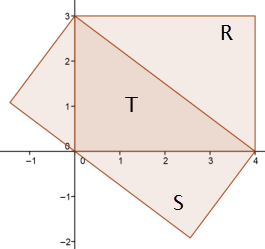
\includegraphics{right-triangle}
    \centering
  \end{figure}

  By \nameref{sec:choice-scale}, both $R$ and $S$ are measurable.
  By this same axiom, $a(R) = ab$ and $a(S) = ca\sin{\theta}$.
  By the \nameref{sec:additive-property}, $R \cup S$ and $R \cap S$ are both
    measurable.
  $a(R \cap S) = a(T)$ and $a(R \cup S)$ can be determined by noting that
    $R$'s construction implies identity $a(R) = 2a(T)$.
  Therefore
    \begin{align*}
      a(T)
        & = a(R \cap S) \\
        & = a(R) + a(S) - a(R \cup S) \\
        & = ab + ca\sin{\theta} - a(R \cup S) \\
        & = ab + ca\sin{\theta} - (ca\sin{\theta} + \frac{1}{2}a(R)) \\
        & = ab + ca\sin{\theta} - ca\sin{\theta} - a(T).
    \end{align*}
  Solving for $a(T)$ gives the desired identity: $$a(T) = \frac{1}{2}ab.$$
  By \nameref{sec:invariance-under-congruence}, $a(T') = a(T)$, concluding our
    proof.

\end{proof}

\section{\unverified{Exercise 1.7.3}}%
\label{sec:exercise-1.7.3}

Prove that every trapezoid and every parallelogram is measurable and derive the
  usual formulas for their areas.

\begin{proof}

  We begin by proving the formula for a trapezoid.
  Let $S$ be a trapezoid with height $h$ and bases $b_1$ and $b_2$, $b_1 < b_2$.
  There are three cases to consider:

  \begin{figure}[h]
    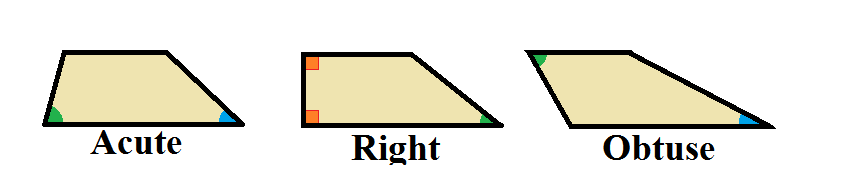
\includegraphics[width=\textwidth]{trapezoid-cases}
    \centering
  \end{figure}

  \paragraph{Case 1}%

    Suppose $S$ is a right trapezoid.
    Then $S$ is the union of non-overlapping rectangle $R$ of width $b_1$ and
      height $h$ with right triangle $T$ of base $b_2 - b_1$ and height $h$.
    By \nameref{sec:choice-scale}, $R$ is measurable.
    By \nameref{sec:exercise-1.7.2}, $T$ is measurable.
    By the \nameref{sec:additive-property}, $R \cup T$ and $R \cap T$ are both
      measurable and
      \begin{align*}
        a(S)
          & = a(R \cup T) \\
          & = a(R) + a(T) - a(R \cap T) \\
          & = a(R) + a(T) & \text{by construction} \\
          & = b_1h + a(T) & \text{Choice of Scale} \\
          & = b_1h + \frac{1}{2}(b_2 - b_1)h & \textref{sec:exercise-1.7.2} \\
          & = \frac{b_1 + b_2}{2}h.
      \end{align*}

  \paragraph{Case 2}%

    Suppose $S$ is an acute trapezoid.
    Then $S$ is the union of non-overlapping triangle $T$ and right trapezoid $R$.
    Let $c$ denote the length of base $T$.
    Then $R$ has longer base edge of length $b_2 - c$.
    By \nameref{sec:exercise-1.7.2}, $T$ is measurable.
    By Case 1, $R$ is measurable.
    By the \nameref{sec:additive-property}, $R \cup T$ and $R \cap T$ are both
      measurable and
      \begin{align*}
        a(S)
          & = a(T) + a(R) - a(R \cap T) \\
          & = a(T) + a(R) & \text{by construction} \\
          & = \frac{1}{2}ch + a(R) & \textref{sec:exercise-1.7.2} \\
          & = \frac{1}{2}ch + \frac{b_1 + b_2 - c}{2}h & \text{Case 1} \\
          & = \frac{b_1 + b_2}{2}h.
      \end{align*}

  \paragraph{Case 3}%

    Suppose $S$ is an obtuse trapezoid.
    Then $S$ is the union of non-overlapping triangle $T$ and right trapezoid $R$.
    Let $c$ denote the length of base $T$.
    Reflect $T$ vertically to form another right triangle, say $T'$.
    Then $T' \cup R$ is an acute trapezoid.
    By \nameref{sec:invariance-under-congruence},
      \begin{equation}
        \label{sec:exercise-1.7.3-eq1}
        \tag{3.1}
        a(T' \cup R) = a(T \cup R).
      \end{equation}
    By construction, $T' \cup R$ has height $h$ and bases $b_1 - c$ and $b_2 + c$
      meaning
      \begin{align*}
        a(T \cup R)
          & = a(T' \cup R) & \eqref{sec:exercise-1.7.3-eq1} \\
          & = \frac{b_1 - c + b_2 + c}{2}h & \text{Case 2} \\
          & = \frac{b_1 + b_2}{2}h.
      \end{align*}

  \paragraph{Conclusion}%

    These cases are exhaustive and in agreement with one another.
    Thus $S$ is measurable and $$a(S) = \frac{b_1 + b_2}{2}h.$$

  \divider

  Let $P$ be a parallelogram with base $b$ and height $h$.
  Then $P$ is the union of non-overlapping triangle $T$ and right trapezoid $R$.
  Let $c$ denote the length of base $T$.
  Reflect $T$ vertically to form another right triangle, say $T'$.
  Then $T' \cup R$ is an acute trapezoid.
  By \nameref{sec:invariance-under-congruence},
    \begin{equation}
      \label{sec:exercise-1.7.3-eq2}
      \tag{3.2}
      a(T' \cup R) = a(T \cup R).
    \end{equation}
  By construction, $T' \cup R$ has height $h$ and bases $b - c$ and $b + c$
    meaning
    \begin{align*}
      a(T \cup R)
        & = a(T' \cup R) & \eqref{sec:exercise-1.7.3-eq2} \\
        & = \frac{b - c + b + c}{2}h & \text{Area of Trapezoid} \\
        & = bh.
    \end{align*}

\end{proof}

\section{Exercise 1.7.4}%
\label{sec:exercise-1.7.4}

Let $P$ be a polygon whose vertices are lattice points.
The area of $P$ is $I + \frac{1}{2}B - 1$, where $I$ denotes the number of
  lattice points inside the polygon and $B$ denotes the number on the boundary.

\subsection{\unverified{Exercise 1.7.4a}}%
\label{sub:exercise-1.7.4a}

Prove that the formula is valid for rectangles with sides parallel to the
  coordinate axes.

\begin{proof}

  Let $P$ be a rectangle with sides parallel to the coordinate axes, with width
    $w$, height $h$, and lattice points for vertices.
  We assume $P$ has three non-collinear points, ruling out any instances of
    points or line segments.

  By \nameref{sec:choice-scale}, $P$ is measurable with area $a(P) = wh$.
  By construction, $P$ has $I = (w - 1)(h - 1)$ interior lattice points and
    $B = 2(w + h)$ lattice points on its boundary.
  The following shows the lattice point area formula is in agreement with
    the expected result:
    \begin{align*}
      I + \frac{1}{2}B - 1
        & = (w - 1)(h - 1) + \frac{1}{2}\left[ 2(w + h) \right] - 1 \\
        & = (wh - w - h + 1) + \frac{1}{2}\left[ 2(w + h) \right] - 1 \\
        & = (wh - w - h + 1) + (w + h) - 1 \\
        & = wh.
    \end{align*}

\end{proof}

\subsection{\unverified{Exercise 1.7.4b}}%
\label{sub:exercise-1.7.4b}

Prove that the formula is valid for right triangles and parallelograms.

\begin{proof}

  Let $P$ be a right triangle with width $w > 0$, height $h > 0$, and lattice
    points for vertices.
  Let $T$ be the triangle $P$ translated, rotated, and reflected such that the
    its vertices are $(0, 0)$, $(0, w)$, and $(w, h)$.
  Let $I_T$ and $B_T$ be the number of interior and boundary points of $T$
    respectively.
  Let $H_L$ denote the number of lattice points on $T$'s hypotenuse.

  Let $R$ be the overlapping rectangle of width $w$ and height $h$, situated
    with bottom-left corner at $(0, 0)$.
  Let $I_R$ and $B_R$ be the number of interior and boundary points
    of $R$ respectively.

  By construction, $T$ shares two sides with $R$.
  Therefore
    \begin{equation}
      \label{sub:exercise-1.7.4b-eq1}
      B_T = \frac{1}{2}B_R - 1 + H_L.
    \end{equation}
  Likewise,
    \begin{equation}
      \label{sub:exercise-1.7.4b-eq2}
      I_T = \frac{1}{2}(I_R - (H_L - 2)).
    \end{equation}
  The following shows the lattice point area formula is in agreement with
    the expected result:
    \begin{align*}
      I_T + \frac{1}{2}B_T - 1
        & = \frac{1}{2}(I_R - (H_L - 2)) + \frac{1}{2}B_T - 1
          & \eqref{sub:exercise-1.7.4b-eq2} \\
        & = \frac{1}{2}\left[ I_R - H_L + B_T \right] \\
        & = \frac{1}{2}\left[ I_R - H_L + \frac{1}{2}B_R - 1 + H_L \right]
          & \eqref{sub:exercise-1.7.4b-eq1} \\
        & = \frac{1}{2}\left[ I_R + \frac{1}{2}B_R - 1 \right] \\
        & = \frac{1}{2}\left[ wh \right] & \textref{sub:exercise-1.7.4a}.
    \end{align*}

  We do not prove this formula is valid for parallelograms here.
  Instead, refer to \nameref{sub:exercise-1.7.4c} below.

\end{proof}

\subsection{\unverified{Exercise 1.7.4c}}%
\label{sub:exercise-1.7.4c}

Use induction on the number of edges to construct a proof for general polygons.

\begin{proof}

  Define predicate $P(n)$ as "An $n$-polygon with vertices on lattice points has
    area $I + \frac{1}{2}B - 1$."
  We use induction to prove $P(n)$ holds for all $n \geq 3$.

  \paragraph{Base Case}%

    A $3$-polygon is a triangle.
    By \nameref{sub:exercise-1.7.4b}, the lattice point area formula holds.
    Thus $P(3)$ holds.

  \paragraph{Induction Step}%

    Assume induction hypothesis $P(k)$ holds for some $k \geq 3$.
    Let $P$ be a $(k + 1)$-polygon with vertices on lattice points.
    Such a polygon is equivalent to the union of a $k$-polygon $S$ with a
      triangle $T$.
    That is, $P = S \cup T$.

    Let $I_P$ be the number of interior lattice points of $P$.
    Let $B_P$ be the number of boundary lattice points of $P$.
    Similarly, let $I_S$, $I_T$, $B_S$, and $B_T$ be the number of interior
      and boundary lattice points of $S$ and $T$.
    Let $c$ denote the number of boundary points shared between $S$ and $T$.

    By our induction hypothesis, $a(S) = I_S + \frac{1}{2}B_S - 1$.
    By our base case, $a(T) = I_T + \frac{1}{2}B_T - 1$.
    By construction, it follows:
      \begin{align*}
        I_P & = I_S + I_T + c - 2 \\
        B_P & = B_S + B_T - (c - 2) - c \\
            & = B_S + B_T - 2c + 2.
      \end{align*}
    Applying the lattice point area formula to $P$ yields the following:
      \begin{align*}
        & I_P + \frac{1}{2}B_P - 1 \\
          & = (I_S + I_T + c - 2) + \frac{1}{2}(B_S + B_T - 2c + 2) - 1 \\
          & = I_S + I_T + c - 2 + \frac{1}{2}B_S + \frac{1}{2}B_T - c + 1 - 1 \\
          & = (I_S + \frac{1}{2}B_S - 1) + (I_T + \frac{1}{2}B_T - 1) \\
          & = a(S) + (I_T + \frac{1}{2}B_T - 1) & \text{induction hypothesis} \\
          & = a(S) + a(T). & \text{base case}
      \end{align*}
    By the \nameref{sec:additive-property}, $S \cup T$ is measurable,
      $S \cap T$ is measurable, and
      \begin{align*}
        a(P)
          & = a(S \cup T) \\
          & = a(S) + a(T) - a(S \cap T) \\
          & = a(S) + a(T). & \text{by construction}
      \end{align*}
    This shows the lattice point area formula is in agreement with our axiomatic
      definition of area.
    Thus $P(k + 1)$ holds.

  \paragraph{Conclusion}%

    By mathematical induction, it follows for all $n \geq 3$, $P(n)$ is true.

\end{proof}

\section{\unverified{Exercise 1.7.5}}%
\label{sec:exercise-1.7.5}

Prove that a triangle whose vertices are lattice points cannot be equilateral.

[\textit{Hint:} Assume there is such a triangle and compute its area in two
ways, using Exercises 2 and 4.]

\begin{proof}

  Proceed by contradiction.
  Let $T$ be an equilateral triangle whose vertices are lattice points.
  Assume each side of $T$ has length $a$.
  Then $T$ has height $h = (a\sqrt{3}) / 2$.
  By \nameref{sec:exercise-1.7.2},
    \begin{equation}
      \label{sub:exercise-1.7.5-eq1}
      \tag{5.1}
      a(T) = \frac{1}{2}ah = \frac{a^2\sqrt{3}}{4}.
    \end{equation}
  Let $I$ and $B$ denote the number of interior and boundary lattice points of
    $T$ respectively.
  By \nameref{sec:exercise-1.7.4},
    \begin{equation}
      \label{sub:exercise-1.7.5-eq2}
      \tag{5.2}
      a(T) = I + \frac{1}{2}B - 1.
    \end{equation}
  But \eqref{sub:exercise-1.7.5-eq1} is irrational whereas
    \eqref{sub:exercise-1.7.5-eq2} is not.
  This is a contradiction.
  Thus, there is \textit{no} equilateral triangle whose vertices are lattice
    points.

\end{proof}

\section{\unverified{Exercise 1.7.6}}%
\label{sec:exercise-1.7.6}

Let $A = \{1, 2, 3, 4, 5\}$, and let $\mathscr{M}$ denote the class of all
  subsets of $A$.
(There are 32 altogether, counting $A$ itself and the empty set $\emptyset$.)
For each set $S$ in $\mathscr{M}$, let $n(S)$ denote the number of distinct
  elements in $S$.
If $S = \{1, 2, 3, 4\}$ and $T = \{3, 4, 5\}$, compute $n(S \cup T)$,
  $n(S \cap T)$, $n(S - T)$, and $n(T - S)$.
Prove that the set function $n$ satisfies the first three axioms for area.

\begin{proof}

  Let $S = \{1, 2, 3, 4\}$ and $T = \{3, 4, 5\}$.
  Then
    \begin{align*}
      n(S \cup T)
        & = n(\{1, 2, 3, 4\} \cup \{3, 4, 5\}) \\
        & = n(\{1, 2, 3, 4, 5\}) \\
        & = 5. \\
      n(S \cap T)
        & = n(\{1, 2, 3, 4\} \cap \{3, 4, 5\}) \\
        & = n(\{3, 4\}) \\
        & = 2. \\
      n(S - T)
        & = n(\{1, 2, 3, 4\} - \{3, 4, 5\}) \\
        & = n(\{1, 2\}) \\
        & = 2. \\
      n(T - S)
        & = n(\{3, 4, 5\} - \{1, 2, 3, 4\}) \\
        & = n(\{5\}) \\
        & = 1.
    \end{align*}
  We now prove $n$ satisfies the first three axioms for area.

  \paragraph{Nonnegative Property}%

    $n$ returns the length of some member of $\mathscr{M}$.
    By hypothesis, the smallest possible input to $n$ is $\emptyset$.
    Since $n(\emptyset) = 0$, it follows $n(S) \geq 0$ for all $S \subset A$.

  \paragraph{Additive Property}%

    Let $S$ and $T$ be members of $\mathscr{M}$.
    It trivially follows that both $S \cup T$ and $S \cap T$ are in
      $\mathscr{M}$.
    Consider the value of $n(S \cup T)$.
    There are two cases to consider:

    \subparagraph{Case 1}%

      Suppose $S \cap T = \emptyset$.
      That is, there is no common element shared between $S$ and $T$.
      Thus
        \begin{align*}
          n(S \cup T)
            & = n(S) + n(T) \\
            & = n(S) + n(T) - 0 \\
            & = n(S) + n(T) - n(S \cap T).
        \end{align*}

    \subparagraph{Case 2}%

      Suppose $S \cap T \neq \emptyset$.
      Then $n(S) + n(T)$ counts each element of $S \cap T$ twice.
      Therefore $n(S \cup T) = n(S) + n(T) - n(S \cap T)$.

    \subparagraph{Conclusion}%

      These cases are exhaustive and in agreement with one another.
      Thus $n(S \cup T) = n(S) + n(T) - n(S \cap T)$.

  \paragraph{Difference Property}%

    Suppose $S, T \in \mathscr{M}$ such that $S \subseteq T$.
    That is, every member of $S$ is a member of $T$.
    By definition, $T - S$ consists of members in $T$ but not in $S$.
    Thus $n(T - S) = n(T) - n(S)$.

\end{proof}

\chapter{Partitions and Step Functions}%
\label{chap:partitions-step-functions}

\section{\defined{Partition}}%
\label{sec:partition}

Let $[a, b]$ be a closed interval decomposed into $n$ subintervals by inserting
  $n - 1$ points of subdivision, say $x_1$, $x_2$, $\ldots$, $x_{n-1}$, subject
  only to the restriction
  \begin{equation}
    \label{sec:partition-eq1}
    a < x_1 < x_2 < \cdots < x_{n-1} < b.
  \end{equation}
It is convenient to denote the point $a$ itself by $x_0$ and the point $b$ by
  $x_n$.
A collection of points satisfying \eqref{sec:partition-eq1} is called a
  \textbf{partition} $P$ of $[a, b]$, and we use the symbol
  $$P = \{x_0, x_1, \ldots, x_n\}$$ to designate this partition.

\begin{definition}

  \lean{Common/Set/Intervals/Partition}{Set.Intervals.Partition}

\end{definition}

\section{\defined{Step Function}}%
\label{sec:step-function}

A function $s$, whose domain is a closed interval $[a, b]$, is called a step
  function if there is a \nameref{sec:partition} $P = \{x_0, x_1, \ldots, x_n\}$
  of $[a b]$ such that $s$ is constant on each open subinterval of $P$.
That is to say, for each $k = 1, 2, \ldots, n$, there is a real number $s_k$
  such that $$s(x) = s_k \quad\text{if}\quad x_{k-1} < x < x_k.$$
Step functions are sometimes called piecewise constant functions.

\vspace{8pt}
\noindent
\textit{Note:} At each of the endpoints $x_{k-1}$ and $x_k$ the function must
  have some well-defined value, but this need not be the same as $s_k$.

\begin{definition}

  \lean{Common/Set/Intervals/StepFunction}{Set.Intervals.StepFunction}

\end{definition}

\chapter{Exercises 1.11}%
\label{chap:exercises-1-11}

\section{Exercise 1.11.4}%
\label{sec:exercise-1.11.4}

Prove that the greatest-integer function has the properties indicated:

\subsection{\verified{Exercise 1.11.4a}}%
\label{sub:exercise-1.11.4a}

$\floor{x + n} = \floor{x} + n$ for every integer $n$.

\begin{proof}

  \lean{Bookshelf/Apostol/Chapter\_1\_11}
    {Apostol.Chapter\_1\_11.exercise\_4a}

  \divider

  Let $x$ be a real number and $n$ an integer.
  Let $m = \floor{x + n}$.
  By definition of the floor function, $m$ is the unique integer such that
    $m \leq x + n < m + 1$.
  Then $m - n \leq x < (m - n) + 1$.
  That is, $m - n = \floor{x}$.
  Rearranging terms we see that $m = \floor{x} + n$ as expected.

\end{proof}

\subsection{\verified{Exercise 1.11.4b}}%
\label{sub:exercise-1.11.4b}

$\floor{-x} =
  \begin{cases}
    -\floor{x} & \text{if } x \text{ is an integer}, \\
    -\floor{x} - 1 & \text{otherwise}.
  \end{cases}$

\begin{proof}

  \ \vspace{6pt}

  \lean{Bookshelf/Apostol/Chapter\_1\_11}
    {Apostol.Chapter\_1\_11.exercise\_4b\_1}

  \lean{Bookshelf/Apostol/Chapter\_1\_11}
    {Apostol.Chapter\_1\_11.exercise\_4b\_2}

  \divider

  There are two cases to consider:

  \paragraph{Case 1}%

    Suppose $x$ is an integer.
    Then $x = \floor{x}$ and $-x = \floor{-x}$.
    It immediately follows that $$\floor{-x} = -x = -\floor{x}.$$

  \paragraph{Case 2}%

    Suppose $x$ is not an integer.
    Let $m = \floor{-x}$.
    By definition of the floor function, $m$ is the unique integer such that
      $m \leq -x < m + 1$.
    Equivalently, $-m - 1 < x \leq -m$.
    Since $x$ is not an integer, it follows $-m - 1 \leq x < -m$.
    Then, by definition of the floor function, $\floor{x} = -m - 1$.
    Solving for $m$ yields $$\floor{-x} = m = -\floor{x} - 1.$$

  \paragraph{Conclusion}%

    The above two cases are exhaustive. Thus
      $$\floor{-x} =
        \begin{cases}
          -\floor{x} & \text{if } x \text{ is an integer}, \\
          -\floor{x} - 1 & \text{otherwise}.
        \end{cases}$$

\end{proof}

\subsection{\verified{Exercise 1.11.4c}}%
\label{sub:exercise-1.11.4c}

$\floor{x + y} = \floor{x} + \floor{y}$ or $\floor{x} + \floor{y} + 1$.

\begin{proof}

  \lean{Bookshelf/Apostol/Chapter\_1\_11}
    {Apostol.Chapter\_1\_11.exercise\_4c}

  \divider

  Rewrite $x$ and $y$ as the sum of their floor and fractional components:
    $x = \floor{x} + \{x\}$ and $y = \floor{y} + \{y\}$.
  Now
    \begin{align}
      \floor{x + y}
        & = \floor{\floor{x} + \{x\} + \floor{y} + \{y\}} \nonumber \\
        & = \floor{\floor{x} + \floor{y} + \{x\} + \{y\}} \nonumber \\
        & = \floor{x} + \floor{y} + \floor{\{x\} + \{y\}}
          & \textref{sub:exercise-1.11.4a} \label{sub:exercise-1.11.4c-eq1}
    \end{align}
  There are two cases to consider:

  \paragraph{Case 1}%

    Suppose $\{x\} + \{y\} < 1$.
    Then $\floor{\{x\} + \{y\}} = 0$.
    Substituting this value into \eqref{sub:exercise-1.11.4c-eq1} yields
      $$\floor{x + y} = \floor{x} + \floor{y}.$$

  \paragraph{Case 2}%

    Suppose $\{x\} + \{y\} \geq 1$.
    Because $\{x\}$ and $\{y\}$ are both less than $1$, $\{x\} + \{y\} < 2$.
    Thus $\floor{\{x\} + \{y\}} = 1$.
    Substituting this value into \eqref{sub:exercise-1.11.4c-eq1} yields
      $$\floor{x + y} = \floor{x} + \floor{y} + 1.$$

  \paragraph{Conclusion}%

    Since the above two cases are exhaustive, it follows
      $\floor{x + y} = \floor{x} + \floor{y}$ or $\floor{x} + \floor{y} + 1$.

\end{proof}

\subsection{\partial{Exercise 1.11.4d}}%
\label{sub:exercise-1.11.4d}

$\floor{2x} = \floor{x} + \floor{x + \frac{1}{2}}.$

\begin{proof}

  \lean{Bookshelf/Apostol/Chapter\_1\_11}
    {Apostol.Chapter\_1\_11.exercise\_4d}

  \divider

  This is immediately proven by applying Hermite's Identity as shown in
    \nameref{sec:exercise-1.11.5}.

\end{proof}

\subsection{\partial{Exercise 1.11.4e}}%
\label{sub:exercise-1.11.4e}

$\floor{3x} = \floor{x} + \floor{x + \frac{1}{3}} + \floor{x + \frac{2}{3}}.$

\begin{proof}

  \lean{Bookshelf/Apostol/Chapter\_1\_11}
    {Apostol.Chapter\_1\_11.exercise\_4e}

  \divider

  This is immediately proven by applying Hermite's Identity as shown in
    \nameref{sec:exercise-1.11.5}.

\end{proof}

\section{\partial{Exercise 1.11.5}}%
\label{sec:exercise-1.11.5}

The formulas in Exercises 4(d) and 4(e) suggest a generalization for
  $\floor{nx}$.
State and prove such a generalization.

\note{The stated generalization is known as "Hermite's Identity."}

\begin{proof}

  \lean{Bookshelf/Apostol/Chapter\_1\_11}
    {Apostol.Chapter\_1\_11.exercise\_5}

  \divider

  We prove that for all natural numbers $n$ and real numbers $x$, the following
    identity holds:
    \begin{equation}
      \label{sec:exercise-1.11.5-eq1}
      \floor{nx} = \sum_{i=0}^{n-1} \floor{x + \frac{i}{n}}
    \end{equation}
  By definition of the floor function, $x = \floor{x} + r$ for some
    $r \in \ico{0}{1}$.
  Define $S$ as the partition of non-overlapping subintervals
    $$\ico{0}{\frac{1}{n}}, \ico{\frac{1}{n}}{\frac{2}{n}}, \ldots,
      \ico{\frac{n-1}{n}}{1}.$$
  By construction, $\cup\; S = \ico{0}{1}$.
  Therefore there exists some $j \in \mathbb{N}$ such that
    \begin{equation}
      \label{sec:exercise-1.11.5-eq2}
      r \in \ico{\frac{j}{n}}{\frac{j+1}{n}}.
    \end{equation}
  With these definitions established, we now show the left- and right-hand sides
    of \eqref{sec:exercise-1.11.5-eq1} evaluate to the same number.

  \paragraph{Left-Hand Side}%

    Consider the left-hand side of identity \eqref{sec:exercise-1.11.5-eq1}.
    By \eqref{sec:exercise-1.11.5-eq2}, $nr \in \ico{j}{j + 1}$.
    Therefore $\floor{nr} = j$.
    Thus
      \begin{align}
        \floor{nx}
          & = \floor{n(\floor{x} + r)} \nonumber \\
          & = \floor{n\floor{x} + nr} \nonumber \\
          & = \floor{n\floor{x}} + \floor{nr}. \nonumber
            & \textref{sub:exercise-1.11.4a} \\
          & = \floor{n\floor{x}} + j \nonumber \\
          & = n\floor{x} + j. \label{sec:exercise-1.11.5-eq3}
      \end{align}

  \paragraph{Right-Hand Side}%

    Now consider the right-hand side of identity
      \eqref{sec:exercise-1.11.5-eq1}.
    We note each summand, by construction, is the floor of $x$ added to a
      nonnegative number less than one.
    Therefore each summand contributes either $\floor{x}$ or $\floor{x} + 1$ to
      the total.
    Letting $z$ denote the number of summands that contribute $\floor{x} + 1$,
      we have
      \begin{equation}
        \label{sec:exercise-1.11.5-eq4}
        \sum_{i=0}^{n-1} \floor{x + \frac{i}{n}} = n\floor{x} + z.
      \end{equation}
    The value of $z$ corresponds to the number of indices $i$ that satisfy
      $$\frac{i}{n} \geq 1 - r.$$
    By \eqref{sec:exercise-1.11.5-eq2}, it follows
      \begin{align*}
        1 - r
          & \in \ioc{1 - \frac{j+1}{n}}{1-\frac{j}{n}} \\
          & = \ioc{\frac{n - j - 1}{n}}{\frac{n - j}{n}}.
      \end{align*}
    Thus we can determine the value of $z$ by instead counting the number of
      indices $i$ that satisfy $$\frac{i}{n} \geq \frac{n - j}{n}.$$
    Rearranging terms, we see that $i \geq n - j$ holds for
      $z = (n - 1) - (n - j) + 1 = j$ of the $n$ summands.
    Substituting the value of $z$ into \eqref{sec:exercise-1.11.5-eq4} yields
      \begin{equation}
        \label{sec:exercise-1.11.5-eq5}
        \sum_{i=0}^{n-1} \floor{x + \frac{i}{n}} = n\floor{x} + j.
      \end{equation}

  \paragraph{Conclusion}%

    Since \eqref{sec:exercise-1.11.5-eq3} and \eqref{sec:exercise-1.11.5-eq5}
      agree with one another, it follows identity
      \eqref{sec:exercise-1.11.5-eq1} holds.

\end{proof}

\section{\unverified{Exercise 1.11.6}}%
\label{sec:exercise-1.11.6}

Recall that a lattice point $(x, y)$ in the plane is one whose coordinates are
  integers.
Let $f$ be a nonnegative function whose domain is the interval $[a, b]$, where
  $a$ and $b$ are integers, $a < b$.
Let $S$ denote the set of points $(x, y)$ satisfying $a \leq x \leq b$,
  $0 < y \leq f(x)$.
Prove that the number of lattice points in $S$ is equal to the sum
  $$\sum_{n=a}^b \floor{f(n)}.$$

\begin{proof}

  Let $i = a, \ldots, b$ and define $S_i = \mathbb{N} \cap \ioc{0}{f(i)}$.
  By construction, the number of lattice points in $S$ is
    \begin{equation}
      \label{sec:exercise-1.11.6-eq1}
      \sum_{n = a}^b \abs{S_n}.
    \end{equation}
  All that remains is to show $\abs{S_i} = \floor{f(i)}$.
  There are two cases to consider:

  \paragraph{Case 1}%

    Suppose $f(i)$ is an integer.
    Then the number of integers in $\ioc{0}{f(i)}$ is $f(i) = \floor{f(i)}$.

  \paragraph{Case 2}%

    Suppose $f(i)$ is not an integer.
    Then the number of integers in $\ioc{0}{f(i)}$ is the same as that of
      $\ioc{0}{\floor{f(i)}}$.
    Once again, that number is $\floor{f(i)}$.

  \paragraph{Conclusion}%

    By cases 1 and 2, $\abs{S_i} = \floor{f(i)}$.
    Substituting this identity into \eqref{sec:exercise-1.11.6-eq1} finishes the
      proof.

\end{proof}

\section{Exercise 1.11.7}%
\label{sec:exercise-1.11.7}

If $a$ and $b$ are positive integers with no common factor, we have the formula
  $$\sum_{n=1}^{b-1} \floor{\frac{na}{b}} = \frac{(a - 1)(b - 1)}{2}.$$
When $b = 1$, the sum on the left is understood to be $0$.

\note{When $b = 1$, the proofs of (a) and (b) are trivial. We continue under the
  assumption $b > 1$.}

\subsection{\unverified{Exercise 1.11.7a}}%
\label{sub:exercise-1.11.7a}

Derive this result by a geometric argument, counting lattice points in a right
  triangle.

\begin{proof}

  Let $f \colon [1, b - 1] \rightarrow \mathbb{R}$ be given by $f(x) = ax / b$.
  Let $S$ denote the set of points $(x, y)$ satisfying $1 \leq x \leq b - 1$,
    $0 < y \leq f(x)$.
  By \nameref{sec:exercise-1.11.6}, the number of lattice points of $S$ is equal
    to the sum
    \begin{equation}
      \label{sub:exercise-1.11.7a-eq1}
      \sum_{n=1}^{b-1} \floor{f(n)} = \sum_{n=1}^{b-1} \floor{\frac{na}{b}}.
    \end{equation}
  Define $T$ to be the triangle of width $w = b$ and height $h = f(b) = a$
    as $$T = \{ (x, y) : 0 < x < b, 0 < y \leq f(x) \}.$$
  By construction, $T$ does not introduce any additional lattice points.
  Thus $S$ and $T$ have the same number of lattice points.
  Let $H_L$ denote the number of boundary points on $T$'s hypotenuse.
  We prove that (i) $H_L = 2$ and (ii) that $T$ has $\frac{(a - 1)(b - 1)}{2}$
    lattice points.

  \paragraph{(i)}%
  \label{par:exercise-1.11.7a-i}

    Consider the line $L$ overlapping the hypotenuse of $T$.
    By construction, $T$'s hypotenuse has endpoints $(0, 0)$ and $(b, a)$.
    By hypothesis, $a$ and $b$ are positive, excluding the possibility of $L$
      being vertical.
    Define the slope of $L$ as $$m = \frac{a}{b}.$$
    $H_L$ coincides with the number of indices $i = 0, \ldots, b$ such that
      $(i, i * m)$ is a lattice point.
    But $a$ and $b$ are coprime by hypothesis and $i \leq b$.
    Thus $i * m$ is an integer if and only if $i = 0$ or $i = b$.
    Thus $H_L = 2$.

  \paragraph{(ii)}%

    Next we count the number of lattice points in $T$.
    Let $R$ be the overlapping retangle of width $w$ and height $h$, situated
      with bottom-left corner at $(0, 0)$.
    Let $I_R$ denote the number of interior lattice points of $R$.
    Let $I_T$ and $B_T$ denote the interior and boundary lattice points of $T$
      respectively.
    By \nameref{sub:exercise-1.7.4b-eq2},
      \begin{align}
        I_T
          & = \frac{1}{2}(I_R - (H_L - 2)) \nonumber \\
          & = \frac{1}{2}(I_R - (2 - 2))
            & \textref{par:exercise-1.11.7a-i} \nonumber \\
          & = \frac{1}{2}I_R. & \label{sub:exercise-1.11.7a-eq2}
      \end{align}
    Furthermore, since both the adjacent and opposite side of $T$ are not
      included in $T$ and there exist no lattice points on $T$'s hypotenuse
      besides the endpoints, it follows
      \begin{equation}
        \label{sub:exercise-1.11.7a-eq3}
        B_T = 0.
      \end{equation}
    Thus the number of lattice points of $T$ equals
      \begin{align}
        I_T + B_T
          & = I_T & \eqref{sub:exercise-1.11.7a-eq3} \nonumber \\
          & = \frac{1}{2}I_R & \eqref{sub:exercise-1.11.7a-eq2} \nonumber \\
          & = \frac{(b - 1)(a - 1)}{2}.
            & \textref{sub:exercise-1.7.4a} \label{sub:exercise-1.11.7a-eq4}
      \end{align}

  \paragraph{Conclusion}%

    By \eqref{sub:exercise-1.11.7a-eq1} the number of lattice points of $S$ is
      equal to the sum $$\sum_{n=1}^{b-1} \floor{\frac{na}{b}}.$$
    But the number of lattice points of $S$ is the same as that of $T$.
    By \eqref{sub:exercise-1.11.7a-eq4}, the number of lattice points in $T$ is
      equal to $$\frac{(b - 1)(a - 1)}{2}.$$
    Thus $$\sum_{n=1}^{b-1} \floor{\frac{na}{b}} = \frac{(a - 1)(b - 1)}{2}.$$

\end{proof}

\subsection{\partial{Exercise 1.11.7b}}%
\label{sub:exercise-1.11.7b}

Derive the result analytically as follows:
By changing the index of summation, note that
  $\sum_{n=1}^{b-1} \floor{na / b} = \sum_{n=1}^{b-1} \floor{a(b - n) / b}$.
Now apply Exercises 4(a) and (b) to the bracket on the right.

\begin{proof}

  \lean{Bookshelf/Apostol/Chapter\_1\_11}
    {Apostol.Chapter\_1\_11.exercise\_7b}

  \divider

  Let $n = 1, \ldots, b - 1$.
  By hypothesis, $a$ and $b$ are coprime.
  Furthermore, $n < b$ for all values of $n$.
  Thus $an / b$ is not an integer.
  By \nameref{sub:exercise-1.11.4b},
    \begin{equation}
      \label{sub:exercise-1.11.7b-eq1}
      \floor{-\frac{an}{b}} = -\floor{\frac{an}{b}} - 1.
    \end{equation}
  Consider the following:
    \begin{align*}
      \sum_{n=1}^{b-1} \floor{\frac{na}{b}}
        & = \sum_{n=1}^{b-1} \floor{\frac{a(b - n)}{b}} \\
        & = \sum_{n=1}^{b-1} \floor{\frac{ab - an}{b}} \\
        & = \sum_{n=1}^{b-1} \floor{-\frac{an}{b} + a} \\
        & = \sum_{n=1}^{b-1} \floor{-\frac{an}{b}} + a.
          & \textref{sub:exercise-1.11.4a} \\
        & = \sum_{n=1}^{b-1} -\floor{\frac{an}{b}} - 1 + a
          & \eqref{sub:exercise-1.11.7b-eq1} \\
        & = -\sum_{n=1}^{b-1} \floor{\frac{an}{b}} - \sum_{n=1}^{b-1} 1 +
          \sum_{n=1}^{b-1} a \\
        & = -\sum_{n=1}^{b-1} \floor{\frac{an}{b}} - (b - 1) + a(b - 1).
    \end{align*}
  Rearranging the above yields
    $$2\sum_{n=1}^{b-1} \floor{\frac{an}{b}} = (a - 1)(b - 1).$$
  Dividing both sides of the above identity concludes the proof.

\end{proof}

\section{\partial{Exercise 1.11.8}}%
\label{sec:exercise-1.11.8}

Let $S$ be a set of points on the real line.
The \textit{characteristic function} of $S$ is, by definition, the function
  $\mathcal{X}_S$ such that $\mathcal{X}_S(x) = 1$ for every $x$ in $S$, and
  $\mathcal{X}_S(x) = 0$ for those $x$ not in $S$.
Let $f$ be a step function which takes the constant value $c_k$ on the $k$th
  open subinterval $I_k$ of some partition of an interval $[a, b]$.
Prove that for each $x$ in the union $I_1 \cup I_2 \cup \cdots \cup I_n$ we have
  $$f(x) = \sum_{k=1}^n c_k\mathcal{X}_{I_k}(x).$$
This property is described by saying that every step function is a linear
  combination of characteristic functions of intervals.

\begin{proof}

  Let $x \in I_1 \cup I_2 \cup \cdots \cup I_n$ and $N = \{1, \ldots, n\}$.
  Let $k \in N$ such that $x \in I_k$.
  Consider an arbitrary $j \in N - \{k\}$.
  By definition of a partition, $I_j \cap I_k = \emptyset$.
  That is, $I_j$ and $I_k$ are disjoint for all $j \in N - \{k\}$.
  Therefore, by definition of the characteristic function,
    $\mathcal{X}_{I_k}(x) = 1$ and $\mathcal{X}_{I_j}(x) = 0$ for all
    $j \in N - \{k\}$.
  Thus
    \begin{align*}
      f(x)
        & = c_k \\
        & = (c_k)(1) + \sum\nolimits_{j \in N - \{k\}} (c_j)(0) \\
        & = c_k\mathcal{X}_{I_k}(x) +
          \sum\nolimits_{j \in N - \{k\}} c_j\mathcal{X}_{I_j}(x) \\
        & = \sum_{k=1}^n c_k\mathcal{X}_{I_k}(x).
    \end{align*}

\end{proof}

\end{document}
